\documentclass{article}

\usepackage{geometry}
\geometry{
	a4paper,
	total={170mm,257mm},
	left=20mm,
	top=20mm,
}

\usepackage[utf8]{inputenc} % allow utf-8 input
\usepackage[T1]{fontenc}    % use 8-bit T1 fonts
\usepackage[hidelinks]{hyperref}       % hyperlinks
\usepackage{url}            % simple URL typesetting
\usepackage{tikz}
\usepackage{dsfont}
\usepackage{amsmath}
\usepackage{array}
\usepackage{authblk}
\usepackage{float}
\usepackage{rotating}
\bibliographystyle{vancouver}
\usepackage[symbol]{footmisc}
\renewcommand{\thefootnote}{\fnsymbol{footnote}}
\usepackage{makecell}

\usepackage{multirow, makecell}
\renewcommand{\arraystretch}{1.7}
\setlength{\tabcolsep}{12pt}

\renewcommand{\thefigure}{S\arabic{figure}}

\title{Supplementary appendix to: \\ {\Large Estimation of SARS-CoV-2 age-specific mortality during the early stages of an epidemic: a modelling study in Hubei, China and northern Italy}}


\author[a]{Anthony Hauser}
\author[a]{Michel J.~Counotte}
\author[b]{Charles C.~Margossian}
\author[c]{Garyfallos Konstantinoudis}
\author[a]{Nicola Low}
\author[a]{Christian L.~Althaus}
\author[a,*]{Julien Riou}
\affil[a]{{\small Institute of Social and Preventive Medicine, University of Bern, Bern, Switzerland}}
\affil[b]{{\small Department of Statistics, Columbia University, New York, NY}}
\affil[c]{{\small MRC Centre for Environment and Health, Department of Epidemiology and Biostatistics, School of Public Health, Imperial College London, London, UK}}
\affil[*] {{\small Corresponding  author (\texttt{julien.riou@ispm.unibe.ch})}}



\begin{document}
	
	\maketitle
	
\tableofcontents

\clearpage
\section{Data}

\subsection{General data}
	Some data and parameter values are not specific to the area considered.
	The mean incubation period was fixed to 5.9 days, following a study of cases and their contacts in Shenzhen, China \cite{Bi2020}.
	The mean time from disease onset to isolation was fixed to 2.4 days, following the same Shenzhen study \cite{Bi2020}.
	Other works have reported very similar values for both periods \cite{lauerincubation,linton2020incubation,backer2020incubation}.
	These durations were transformed into rates by taking the inverse and used in the system of ordinary differential equations (section \ref{model}).
	As such, this results in exponential distributions of incubation times and time from disease onset to isolation, which is acceptable considering the aim of the SEIR model in this context: obtain a good description of case incidence by date of disease onset in each age class.
	
	Conversely, one of the main objectives of this work was to account for bias due to the delay between disease onset and death.
	For the time from disease onset to death, we used a log-normal distribution with mean 20.2 and standard deviation 11.6 estimated from patient data and accounting from right-censoring \cite{linton2020incubation}.
	We considered other mean durations in sensitivity analyses (section \ref{sst}).
	This continuous probability distribution was discretized by day in order to be used in the model (Figure \ref{fig:distribution_onset_to_death}).
	
\begin{figure}[H]
		\centering
		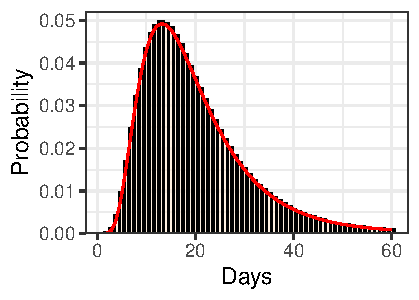
\includegraphics[width=7cm]{../format_output/figures/distribution_onset_to_death.pdf}
		\caption{Probability density function of the time from disease onset to death (red) and corresponding discretization by day between 1 and 60 days (columns).}
		\label{fig:distribution_onset_to_death}
\end{figure}

\subsection{Data from Hubei, China}
We model the dynamics of the COVID-19 epidemic in Hubei from January 1st to February 11th, 2020, considering the introduction of strong control measures from January 20th \cite{jointmission}. 
Our analysis was based on a report published by the Chinese CDC describing all Chinese COVID-19 cases reported up to February 11th, 2020 \cite{Team2020}.
From these reports, we extracted the consolidated number of confirmed cases of COVID-19 {\em by day of disease onset}, the number of deaths per day, and the age distributions of cases and deaths on 11 February 2020 (Figure \ref{fig:china_case_incidence.pdf}).
We also used data about the age distribution of the Chinese population, and about the daily number of potentially infectious contacts by age group in Shanghai \cite{zhang2019patterns}, which we assumed were similar to the population of Hubei.

\begin{figure}[h]
		\centering
		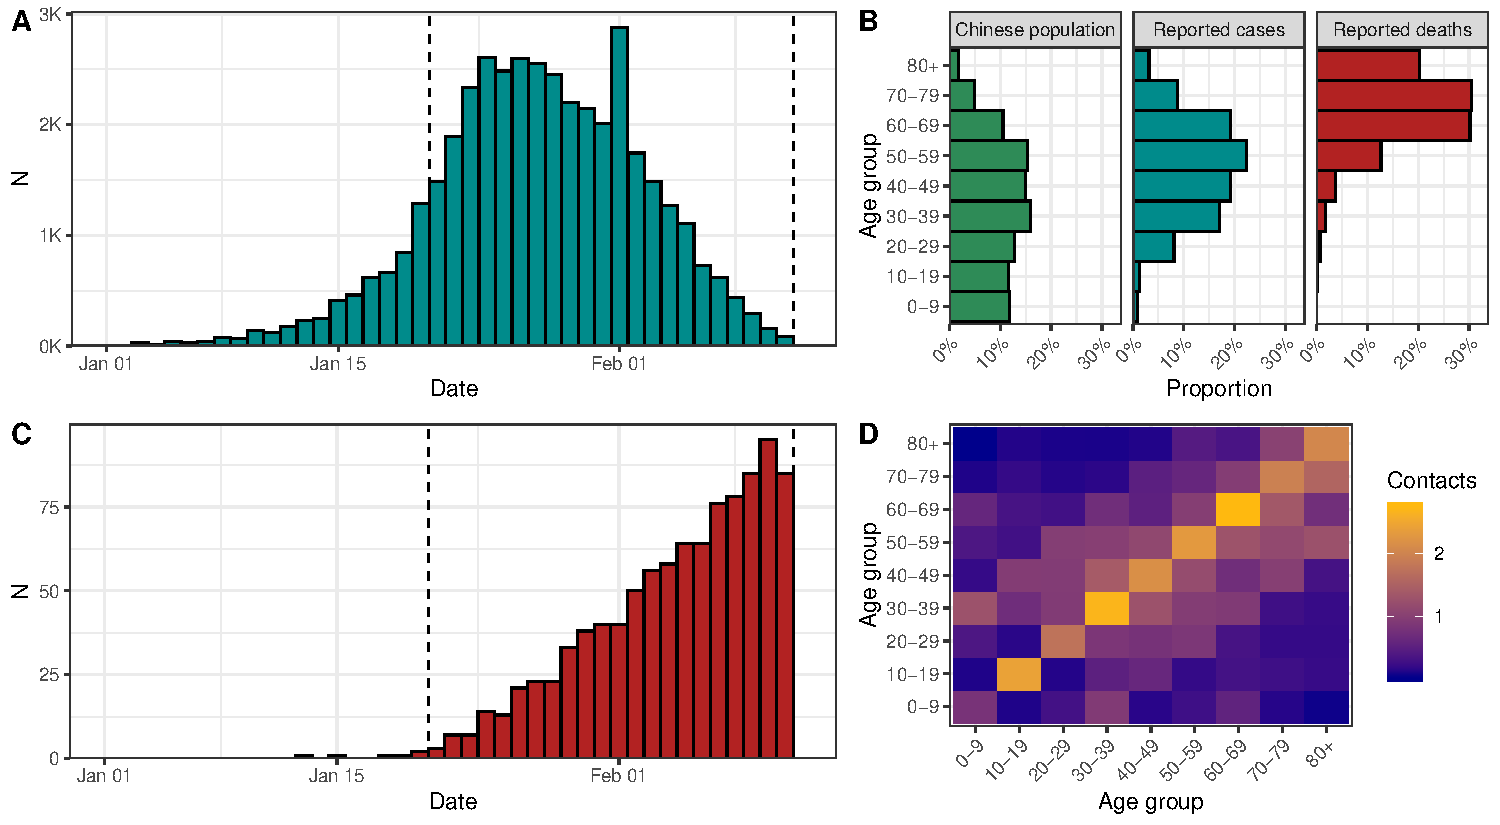
\includegraphics[width=15cm]{../format_output/figures/data_china2.pdf}
		\caption{Data used to fit the model in Hubei, China. (A) Reported confirmed cases of COVID-19 in Hubei by date of disease onset until 11 February, 2020. (B) Age distribution of the Chinese population compared to that of confirmed cases and of deaths due to COVID-19. (C) Reported deaths until 11 February, 2020. (D) Matrix representing the average number of daily contacts between each age class in Shanghai (source: Zhang et al., 2019 \cite{zhang2019patterns}).}
		\label{fig:china_case_incidence.pdf}
\end{figure}

We also extracted data on the proportion of comorbidities among reported COVID-19 cases and deaths \cite{Team2020}.
Age-specific prevalences of diabetes, chronic respiratory diseases, cardiovascular diseases and hypertension in China were extracted from the IHME website \cite{ihme} (Figure \ref{fig:comorbidities}).

\begin{figure}[h]
	\centering
	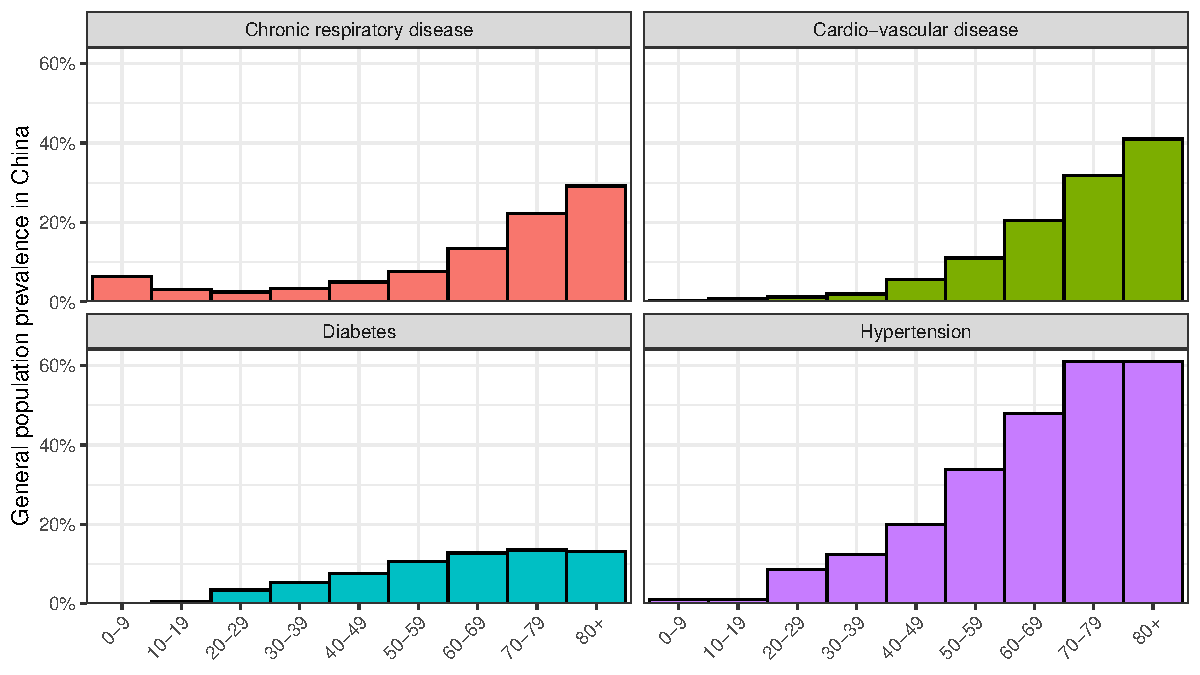
\includegraphics[width=12cm]{../format_output/figures/comorbidity_china.pdf}
	\caption{General population prevalence of four comorbidities by age class in China (source: IHME). }
	\label{fig:comorbidities}
\end{figure}


\subsection{Data from Northern Italy}
We model the dynamics of the COVID-19 epidemic in Northern Italy from 8 February to 3 March, 2020. Our analysis was based on reports from the Instituto Superiore di Sanita and the Dipartimento della Protezione Civile describing all Italian COVID-19 cases reported up to 3 February, 2020 \cite{Civile,IstitutoSuperiorediSanita}. From these reports, we extracted the consolidated number of confirmed cases of COVID-19 {\em by day of disease onset}, the number of deaths per day, and the age distributions of cases and deaths at 15 March 2020 (Figure \ref{fig:italy_case_incidence.pdf}). 
We also collected data about the age distribution of the Italian population \cite{Worldometers.info}, as well as its contact patterns by age group using results from the POLYMOD study \cite{mossong2008social}.
	
	
	\begin{figure}[h]
		\centering
		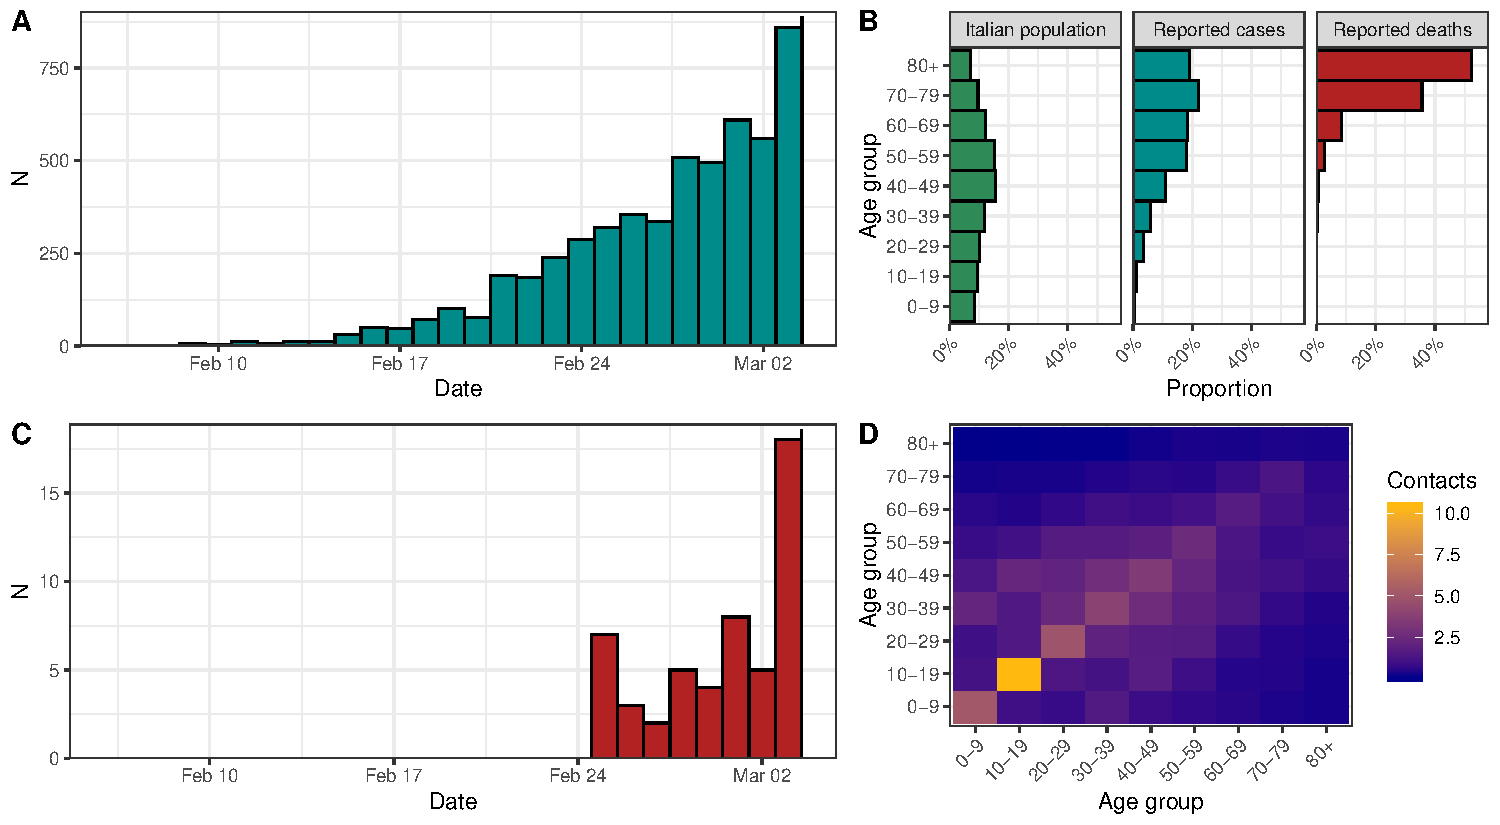
\includegraphics[width=15cm]{../format_output/figures/data_italy.pdf}
		\caption{Data used to fit the model. (A) Reported confirmed cases of COVID-19 in Italy by date of disease onset until 11 February, 2020 (blue), (B) Age distribution of the Italian population compared to that of confirmed cases and of deaths due to COVID-19. (C) Reported deaths in Italy until 11 February, 2020 (red). (D) Matrix representing the number of daily contacts between each age class.}
		\label{fig:italy_case_incidence.pdf}
	\end{figure}
	
	
			\begin{table}[h]
		\centering
		\begin{tabular}{cp{7cm}ll>{\raggedright\arraybackslash}p{2cm}}
			\hline
			Symbol & Comment & Value & Unit & Source \\
			\hline 
			$\mathds{A}$ & Reported cases of COVID-19 in Hubei from 1 January to 11 February 2020 and in Italy from 8 February to 3 March & see Fig \ref{fig:china_case_incidence.pdf}A \& \ref{fig:italy_case_incidence.pdf}A & - & Hubei: \cite{Team2020}, Italy: \cite{Civile,IstitutoSuperiorediSanita}\\
			$\mathds{B}$ & Age distribution of all confirmed cases in China up to 11 February 2020\textsuperscript{*} and in Northern Italy up to 15 March 2020 & see Fig \ref{fig:china_case_incidence.pdf}B \& \ref{fig:italy_case_incidence.pdf}B & - & Hubei: \cite{Team2020}, Italy: \cite{Civile,IstitutoSuperiorediSanita} \\
			$\mathds{C}$ & Deaths among patients with confirmed COVID-19 infection by day of report in China from 1 January to 11 February 2020 \textsuperscript{\dag} and in Nothern Italy from 8 February to 3 March & see Fig \ref{fig:china_case_incidence.pdf}C \& \ref{fig:italy_case_incidence.pdf}C & - & Hubei: \cite{Team2020}, Italy: \cite{Civile,IstitutoSuperiorediSanita} \\
			$\mathds{D}$ & Age distribution of the deaths among patients with confirmed COVID-19 infection that occurred in China up to 11 February 2020 and in Nother Italy up to 15 March \textsuperscript{\ddag} & see Fig \ref{fig:china_case_incidence.pdf}B \& \ref{fig:italy_case_incidence.pdf}B & - & Hubei: \cite{Team2020}, Italy: \cite{Civile,IstitutoSuperiorediSanita} \\
			$\mathds{E}$ & Age distribution of the population in China and Northern Italy & see Fig \ref{fig:china_case_incidence.pdf}B \& \ref{fig:italy_case_incidence.pdf}B & - & \cite{Worldometers.info,UNCTAD} \\
			$\mathds{F}$ & $9\times 9$ matrix with contacts between each age class in Shanghai (used for China) and in Europe (POLYMOD, used for Italy) &  see Fig\ref{fig:china_case_incidence.pdf}D \& \ref{fig:italy_case_incidence.pdf}D & per day & \cite{Zhang2019,mossong2008social} \\  
			$\mathds{G}$ & Distribution of time from disease onset to death & $\text{log-}\mathcal{N}(20.2,11.6)$ & days & \cite{Linton2020a} \\
			$1/\tau$ & Incubation period & 5.9 & days &  \cite{Bi2020} \\
%			$\psi$ & Proportion of symptomatics & $\text{Beta}(71,18)$ & - & \cite{Bi2020} \\
			$1/\mu$ & Time from disease onset to isolation & 2.4 & days & \cite{Bi2020} \\
			$\gamma$ & Time from disease onset to death (mean - standard deviation) & 20.2 - 11.6 & days & \cite{Linton2020} \\
			\hline \\[-2.5em]
			\multicolumn{5}{p{18cm}}{\small{\textsuperscript{*}As 85\% of these are in Hubei, we assume that the age distribution is the same in overall China. \textsuperscript{\dag} As 95\% of these are in Hubei, the numbers were scaled down by 5\%. \textsuperscript{\ddag} We assume that the age distribution is the same in overall China.}}
		\end{tabular} 
		\caption{Summary of data sources and fixed parameters.}\label{data_table}
	\end{table}


	
	\clearpage
	\section{Model}
	\label{model}
	
	We developed an approach aimed at estimating the true mortality associated with COVID-19.
	With regards to a specific epidemic, the model relies upon data on cases by date of disease onset (which is difficult to obtain), mortality by date of death, and the age distribution of both cases and deaths.
	In a first step, we use an age-stratified susceptible-exposed-infected-removed (SEIR) compartmental model to describe the dynamics of transmission of the virus in the population of Hubei, including the decrease in incidence after the introduction of control measures on 20 January.
	In a second step, we estimate the mortality of infected individuals with regards to the probability of dying upon infection and the delay between symptom onset and death. 
	We fit the model to data on the time dynamics and the age distribution of both reported cases and deaths.
	We implemented the model in a Bayesian framework using Stan. 
	All code and data are available from \underline{\smash{\url{https://github.com/jriou/covid_adjusted_cfr/}}}.
	We applied this approach to COVID-19 epidemics in two different settings where appropriate data is available: Hubei (China) and Northern Italy.
	
	
	\subsection{Transmission model structure}
	
	We use an age-stratified susceptible-exposed-infected-removed (SEIR) compartmental model using ordinary differential equations (ODEs), with a distinction between asymptomatic and symptomatic infections. 
	We stratify the population in nine ten-year age groups ($0-9, 10-19, \ldots, 70-79, 80+$). 
	The population of each age group $k$ is divided into five compartments: susceptible ($S_k$), incubating or exposed ($E_k$), infected with symptoms ($I_k$), infected and asymptomatic ($A_k$), and removed ($R_k$).
	Note that the number of individuals in each compartment is scaled by the total population of the area (59,020,000 for Hubei, 25,276,000 for Lombardia, Emilia Romagna, Veneto, Marche and Piemonte), so that the sum of all compartments is 1.
	Since we focus on the first wave of infection in Hubei and the early stage of the epidemic in northern Italy, the total size of the population has a very small impact on the transmission dynamics.
	Susceptible individuals may become infected through contacts with infected individuals with symptoms (assuming that incubating or asymptomatic individuals are not infectious) from any other age group.
	The force of infection $\lambda_k$ depends on the added number of infectious individuals in each age class, weighted by a contact matrix $\mathds{F}$ and the proportion of infection upon contact with an infectious individual $\beta$.
	
	In addition, we include a time-dependent forcing function to account for the reduction in transmissibility following the introduction of control measures in Hubei on 20 January 2020 in Hubei. In northern Italy, this effect is ignored as strict control measures were implemented on 9 March 2020, after the period of interest.
	We model the progressive introduction of control measures using the following logistic function:
	\begin{equation}
	f(t,\eta,\nu, \xi) = \eta + \frac{1-\eta}{1+e^{\xi(t-t_c-\nu)}}
	\end{equation}
	where $\eta$ is the relative reduction in transmission after control measures are fully implemented, $\xi$ is the slope of the logistic function modelling the implementation of the control measures, and $\nu$ is the delay (in days after $t_c$, corresponding to 20 January 2020) until the control measures are 50\% effective.
	
	The force of infection $\lambda_k$ can then be expressed as:
	\begin{equation}
	\lambda_k(t) = f(t,\eta,\nu, \xi) \beta S_k(t) \sum_{l=1}^9  \dfrac{I_l(t)}{\mathds{E}_l}  \mathds{F}_{k,l} 
	\end{equation}
	
	\begin{figure}[H]
		\centering
		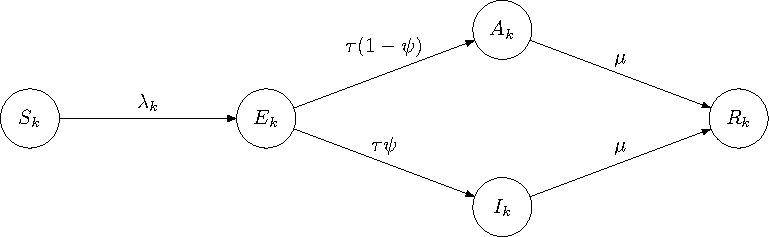
\includegraphics[width=.7\linewidth]{../format_output/figures/fig_ode.pdf}
		\caption{Schematic description of the COVID-19 transmission model. The dashed circles represent the dummy compartments used to record cumulative incidences in asymptomatic and symptomatic people.}
		\label{fig:ode}
	\end{figure}
	
	After the incubation period $1/\tau$, a proportion $\psi$ of infected people develop symptoms and become infectious while the remaining remain asymptomatic and do not transmit the disease further. 
	After a period $1/\mu$, individuals with symptoms are identified and isolated, and thus removed from being infectious.
	The infection dynamics are thus controlled by 4 parameters: $\{\beta,\tau, \psi, \mu \}$.
	
	\subsection{Initial conditions and simulation settings}
	
	The simulation start ($t=0$) is set on the day before the first data point (31 December 2019 for Hubei, 7 February 2020 for northern Italy).
	At this date, most individuals are assumed to be susceptible and are distributed across age groups according to the population age distribution $\mathds{E}$.
	The number of people in the exposed compartments at $t=0$ is controlled by a parameter $\pi$, and also distributed according to $\mathds{E}$.
	Other compartments are set to 0.
	
	\subsection{Dummy compartments and outputs}
	
	In addition to the five compartments per age group, we add two dummy compartments to record the cumulative incidence of new symptomatic infections by day of disease onset, $C_k$:
	\begin{equation}
	\frac{dC^I_k}{dt} = \tau \psi E_k
	\end{equation}
	and the cumulative incidence of new asymptomatic infections, $D_k$:
	\begin{equation}
	\frac{dC^A_k}{dt} = \tau (1- \psi) E_k
	\end{equation}
	Moreover, we need the following outputs in order to fit the model:
	\begin{itemize}
	\item the number of new symptomatic infections per day and by age group:
	\begin{equation}
	\Delta C_{k,t}^{I} =  C^I_k(t) - C^I_k(t-1) 
	\end{equation}
	\item the total number of new infections per day:
	\begin{equation}
	\Delta	C_t^{I} = \sum_k^9 \Delta C_{k,t}^{I}
	\end{equation}	

	\item the total number of new reported infections per day, introducing the age-specific ascertainment proportion parameter $\rho_k$:
	\begin{equation}
		R_t = \sum_k^9 \rho_k \Delta C_{k,t}^{I}
	\end{equation}	
	\item the age distribution of all reported cases up to $t_{\text{max}}=$ 11 February 2020 in Hubei and up to $t_{\text{max}}=$ 3 March in northern Italy:
	\begin{equation}
		D_k^{\text{cases}} =  \frac{\rho_k C^I_k(t_{\text{max}})}{\sum_k^9 \rho_k C^I_k(t_{\text{max}})}
	\end{equation}
	where $t_{\text{max}++}$ represent the index of the last simulated day.
	\end{itemize}

To allow identifiability of the parameters, we remove a degree of freedom by fixing the ascertainment proportion of the highest age group $\rho_9$ to 100\%. 
This assumes that all individuals aged 80 and more that are infected with symptoms seek medical care, are identified and reported to the authorities. 
The ascertainment proportions for other groups $\rho_{1,\ldots,8}$ are estimated from data.

\subsection{Delayed mortality}

Mortality is considered outside of the system of ODEs, using an age-specific mortality parameter $\epsilon_k$.
In accordance to data, we only consider the mortality {\em among cases with a date of disease onset during the period of interest}, up to $t_{\text{max}}=$ 11 February 2020 for Hubei and to $t_{\text{max}}=$ 8 March 2020 for Italy. 
We calculated the mortality until 60 days after the last date of disease onset for each country. 
To do so, we generated a discretized distribution of time from disease onset to death $\mathds{G}$ of length 60 (Figure \ref{fig:distribution_onset_to_death}).\\
To fit the model and to estimate $\epsilon_k$, we need the following mortality-related outputs:	
	\begin{itemize}
		\item the  number of deaths in age group $k$ among people infected before $t_{\text{max}}$ and 60 days after $t_{\text{max}}$, to account for the delay between disease onset and deaths:
		\begin{equation}
		M_{k,t}= \epsilon_k\sum_d^{60}  \Delta C_{k,t-d} \mathds{G}_d 
		\end{equation}
		\item the daily number of deaths summed over age groups, assuming that all deaths are reported:
		\begin{equation}
		M_{t}= \sum_k^9 M_{k,t}
		\end{equation}
		\item the age distribution of all deaths occurring up to $t_{\text{max}}$:
		\begin{equation}
		D_k^{\text{deaths}} = \frac{\sum_{t=1}^{t_{\text{max}}} M_{k,t}}{ \sum_{t=1}^{t_{\text{max}}} M_{t}}
		\end{equation}
	\end{itemize}
	
	
	\subsection{Inference}
	
	The objective of this step is to estimate the following parameters: $\theta=\{\beta, \eta, \xi, \nu, \psi, \pi, \rho_k, \epsilon_k, \phi_1, \phi_2 \}$. We set weakly-informative priors for most of these parameters, which are summarized in Table \ref{prior}.
	For the proportion of symptomatic infections $\phi$, we used an informative prior distribution $\psi \sim \text{Beta}(522,114)$ corresponding to an estimate of 82.1\% (95\% central range: 79.8-84.5) \cite{mizumoto2020estimating}. Implementing this information as a beta distribution allowed the propagation of uncertainty on $\psi$ into the final estimates. For the initial proportion of infected, we used an informative prior distribution $\pi \sim \text{Beta}(1,999)$ corresponding to a 95\% central range of 0-0.0037 of the total population. This range is actually quite large and weakly-informative as it corresponds to a number of initial infections at $t=0$ in the range $[0-640]$.
	
	\begin{table}[h]
		\centering
		\begin{tabular}{cp{8cm}ll}
			\hline
			Symbol & Comment & Support & Prior \\
			\hline 
			$\beta$ & Probability of transmission upon contact & $[0-1]$ & $\text{Beta}(1,1)$  \\
			$\eta$ & Reduction in transmission after control measures & $[0-1]$ & $\text{Beta}(1,1)$ \\
			$\xi$ & Slope of logistic function for control measures implementation & $[0.5-1.5]$ & $ \text{Beta}(1,1) + 0.5$  \\
			$\nu$ & Shift of logistic function for control measures implementation & $[0-\infty[$ & $\text{Exp}(1)$  \\
			$\psi$ & Proportion of symptomatics of 82\% on the Diamond Princess \cite{diamond2} & $$[0-1]$$ & $\text{Beta}(522,114)$ \\
%			 & OR of 80\% among contacts of cases in Shenzen \cite{Bi2020} & $$[0-1]$$ & $\text{Beta}(71,18)$ \\
			$\epsilon_k$ & Proportion of deaths among symptomatic cases (by age group) & $$[0-1]$$ & $\text{Beta}(1,1)$  \\
			$\rho_k$ & Reporting rate of symptomatic cases (by age group) & $$[0-1]$$ & $\text{Beta}(1,1)$  \\
			$\pi$ & Initial proportion of exposed (at $t=0$) & $$[0-1]$$ & $\text{Beta}(1,999)$  \\
			$\phi_1$ & Overdispersion for cases & $[0-\infty[$ & $\text{Exp}(1/100)$  \\
			$\phi_2$ & Overdispersion for deaths & $[0-\infty[$ & $\text{Exp}(1/100)$  \\
			
			\hline 
		\end{tabular} 
		\caption{Summary of parameters.}\label{prior}
	\end{table}
	

We simultaneously fitted our model to four data sets: 
	\begin{enumerate}
		\item the number of reported cases of COVID-19 by day of disease onset:
		\begin{equation}
		\Pr(\theta| \mathds{A}) = \text{Neg-Bin}(\mathds{A}| R_t,\phi_1)
		\end{equation}
		
		\item the age distribution of all confirmed cases up at $t_{\text{max}}$:
		\begin{equation}
		\Pr(\theta| \mathds{B}) = \text{Multinomial}(\mathds{B}|D_k^{\text{cases}})
		\end{equation}
		
		\item the number of deaths among patients with confirmed COVID-19 infection by day of report:
		\begin{equation}
		\Pr(\theta| \mathds{C}) = \text{Neg-Bin}(\mathds{C}|M_t,\phi_2)
		\end{equation}
		
		\item the age distribution of the deaths among patients with confirmed COVID-19 infection that occurred before $t_{\text{max}}$:
		\begin{equation}
		\Pr(\theta| \mathds{D}) = \text{Multinomial}(\mathds{D}|D_k^{\text{deaths}})
		\end{equation}
	\end{enumerate}
	This leads to the following likelihood:
	\begin{equation}
	\Pr(\theta | \mathds{A},\mathds{B},\mathds{C},\mathds{D}) = \Pr(\theta| \mathds{A}) \cdot \Pr(\theta| \mathds{B}) \cdot \Pr(\theta| \mathds{C}) \cdot \Pr(\theta| \mathds{D})
	\end{equation}
	
\subsection{Estimates of mortality}
Table \ref{tab_cfr} summarizes the different estimates of mortality according to whether we adjust for preferential ascertainment of severe cases and/or right-censoring of deaths.


\begin{table}[H]
		\centering
		\begin{tabular}{cc|cc}
			

		 & & \multicolumn{2}{c}{Adjusting for preferential ascertainment}\\
		 & & No & Yes \\[3pt]
		 \hline
		\multirowcell{3}{Adjusting for\\[2pt] right-censoring of deaths} & No & $\dfrac{ M_{t_{\text{max}}}}{ R_{t_{\text{max}}}}$ & $\dfrac{ M_{t_{\text{max}}}}{ C_{t_{\text{max}}}^{I}}$\\[20pt]
		& Yes & $\dfrac{ M_{t_{\text{max}}+60}}{ R_{t_{\text{max}}+60}}$ & $\dfrac{ M_{t_{\text{max}}+60}}{ C_{t_{\text{max}}+60}^{I}}$\\[10pt]

%		\\[-10pt]
		\end{tabular}
		\caption{Mortality among symptomatic infections.}
		\label{tab_cfr}
\end{table}
We also estimate the adjusted mortality in the overall infected (symptomatic or asymptomatic) population:
\begin{equation}
\dfrac{ M_{t_{\text{max}}+60}}{ C_{t_{\text{max}}+60}^{I}+C_{t_{\text{max}}+60}^{A}}
\end{equation}	

\subsection{Implementation and diagnostics}
\label{diag}

We implemented the model in \textit{Stan} \cite{Carpenter2017}, that uses Hamiltonian Monte Carlo sampling.
We estimated the posterior distributions by sampling 500 iterations after 500 iterations for warm-up in four independent chains.
We assessed convergence visually and by using the Gelman-Rubin convergence diagnostic $\hat{R}$.
We also checked for divergent transitions.

Mixing of chains was good in both Hubei and northern Italy (Figures \ref{fig:trace1} and \ref{fig:trace2}), with a maximal $\hat{R}$ of 1.011 in Hubei and 1.006 in northern Italy, more than 500 effective sample size and no divergent transition.
	
	\begin{figure}[H]
	\centering
	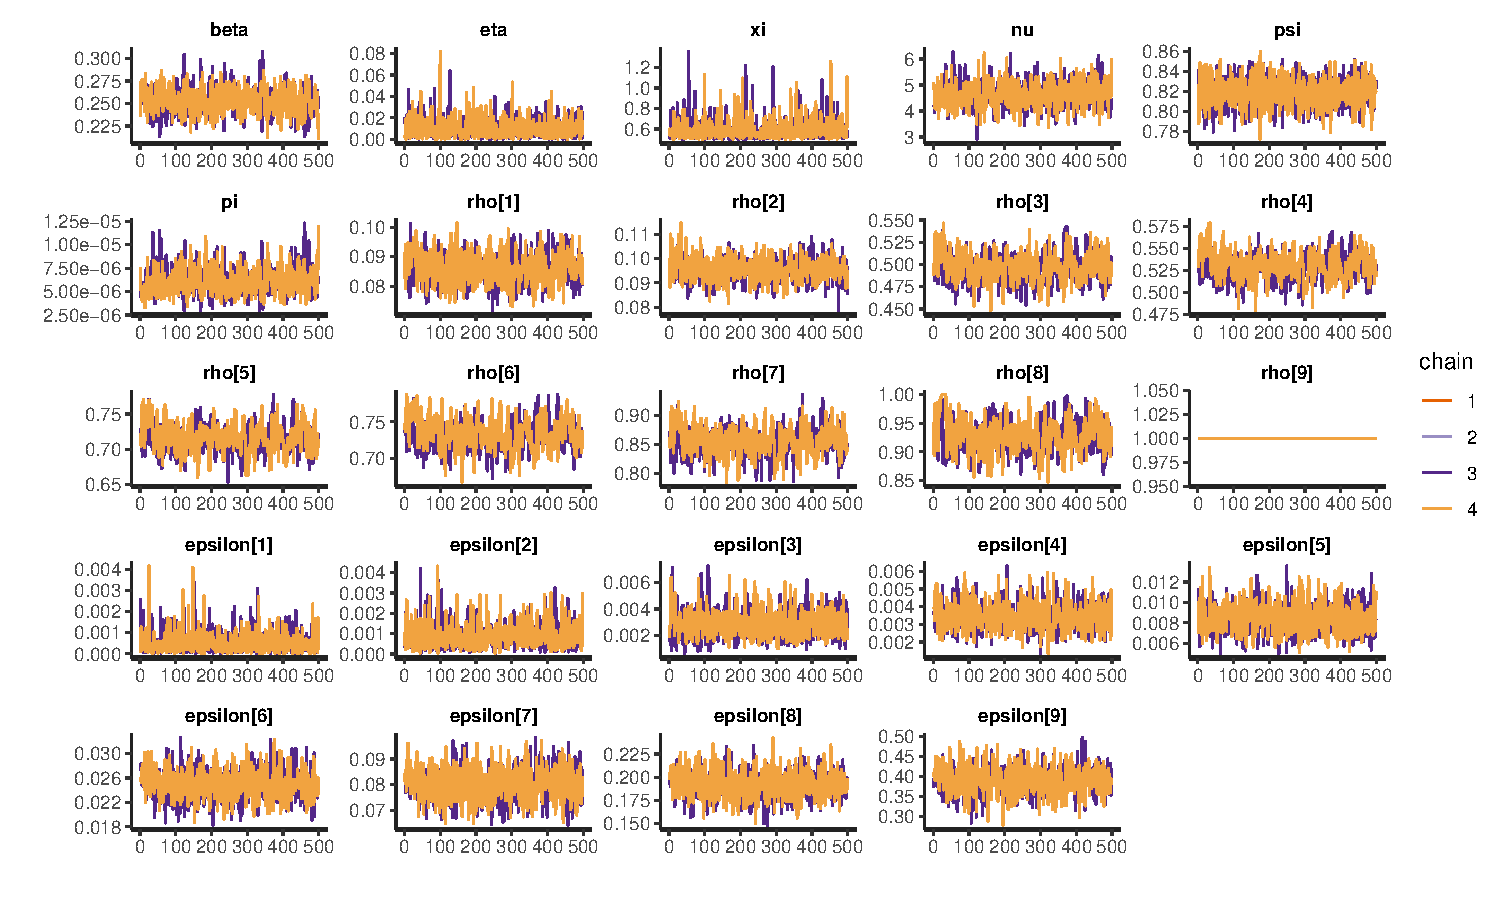
\includegraphics[width=\linewidth]{../format_output/figures/traceplot_china.pdf}
	\caption{Trace plot of the model parameters in Hubei, China.}
	\label{fig:trace1}
	\end{figure}
		
	\begin{figure}[H]
		\centering
		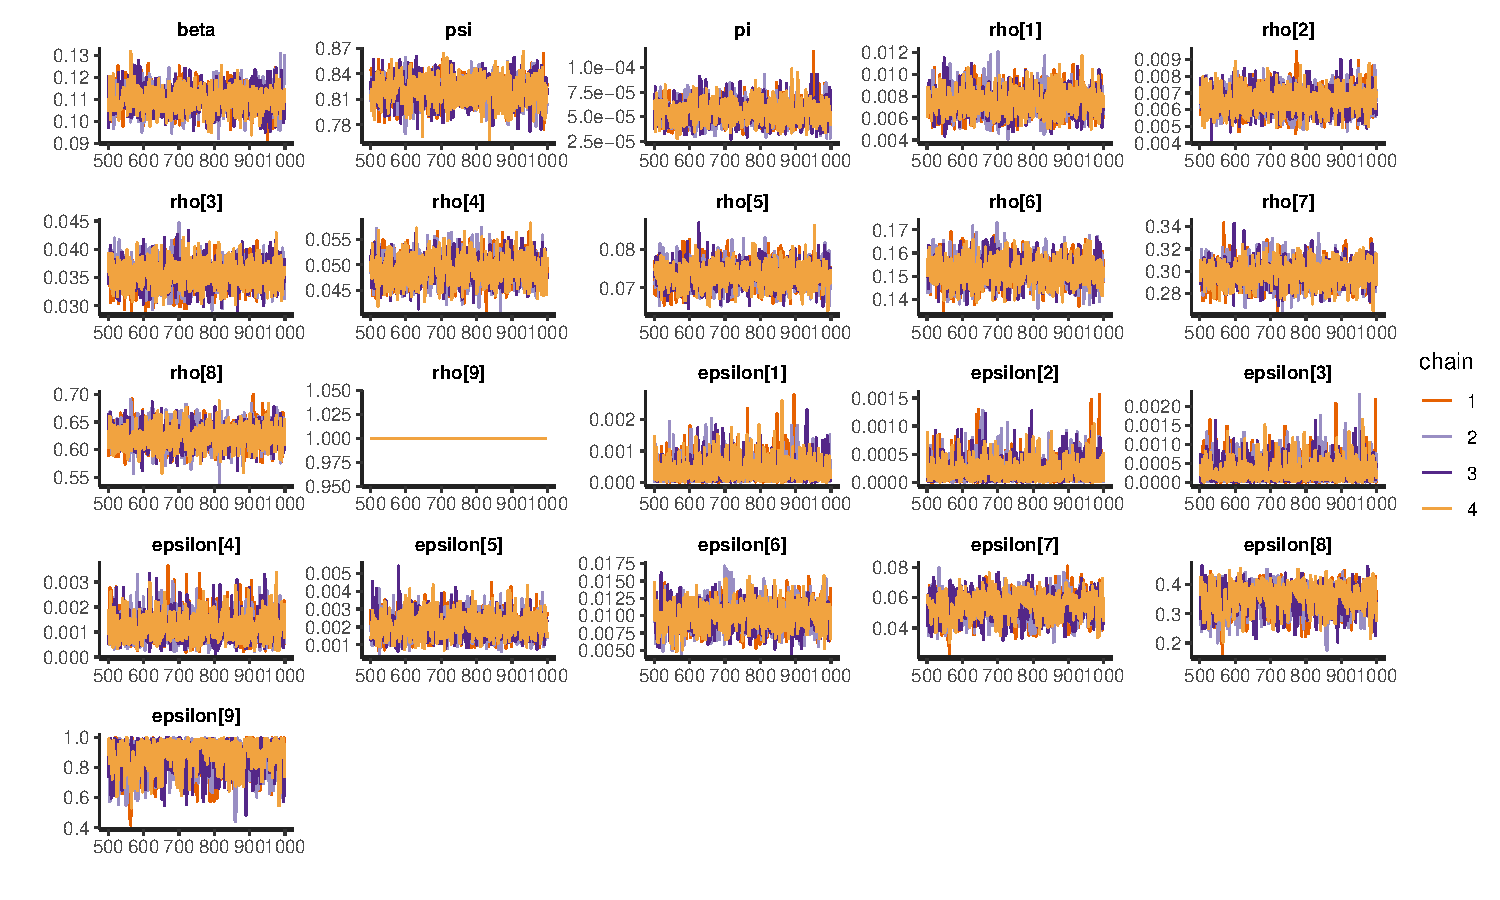
\includegraphics[width=\linewidth]{../format_output/figures/traceplot_italy.pdf}
		\caption{Trace plot of the model parameters in northern Italy.}
		\label{fig:trace2}
	\end{figure}

\clearpage
\section{External validation}

Some level of external validation of our approach for correcting right-censoring in deaths could be conducted using later reports of deaths in Hubei, China (Figure \ref{fig:mortality}).
Visual comparison shows that prediction of deaths align well with later reports (triangles), especially if we average with zero deaths with days with a large number of reported deaths.
An important caveat of this comparison is that model prediction only concerns deaths among people infected before 11 February, while later reported deaths may also concern people infected after this date.
In Hubei, as the model captured the epidemic wave almost until the end, this effect is less important, but this is why external validation was not conducted for northern Italy.
In any case, the good alignment of predictions and later death reports may serve as an external indication of the adequacy of the model, especially regarding the time between disease onset and deaths (this can be compared with a sensitivity analysis using a shorter duration from disease onset to death, see section \ref{sst}).

\begin{figure}[H]
	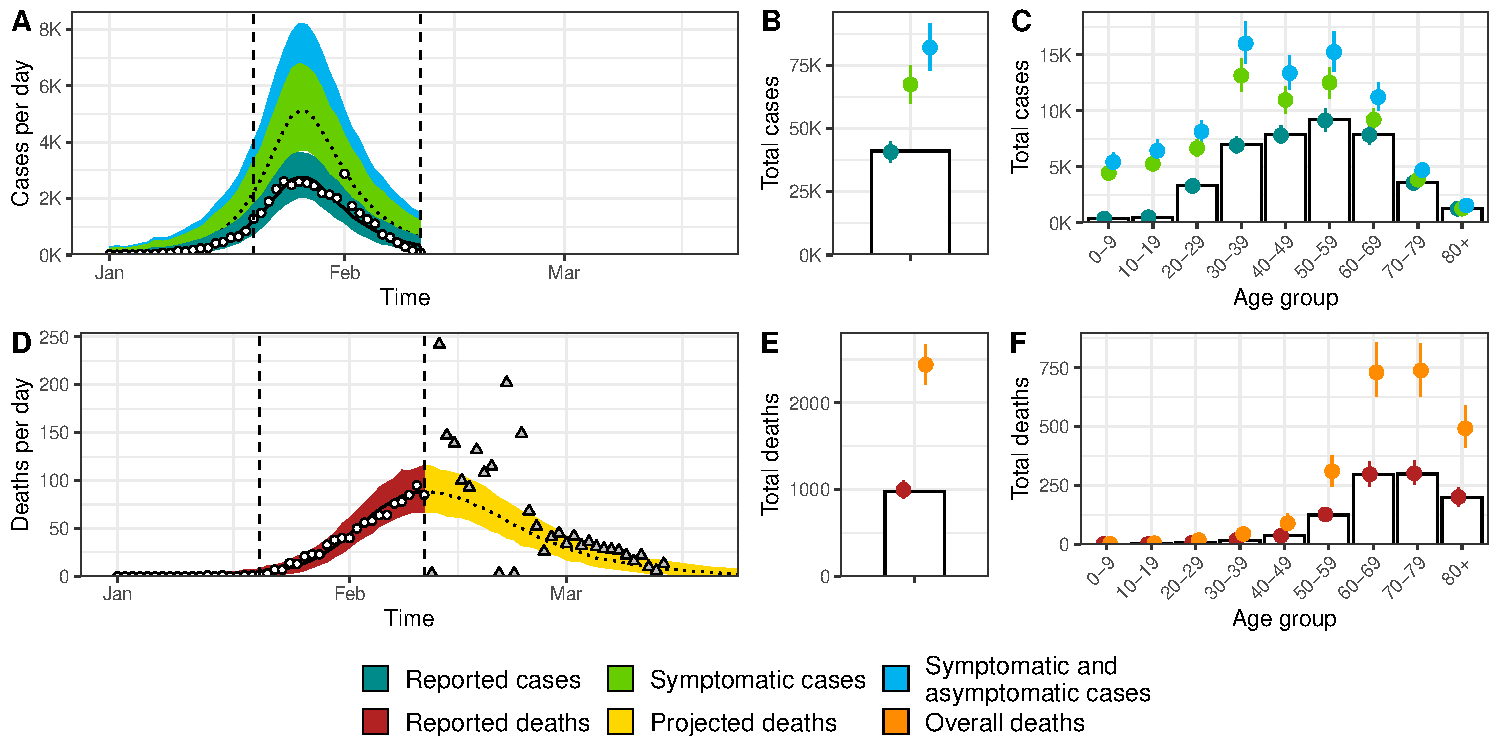
\includegraphics[width=\linewidth]{../format_output/figures/modelfit_china_bis.pdf}
\caption{Model fit for Hubei, China of (A) incident cases of SARS-CoV-2 infection by date of disease onset, (B) total cases, (C) age distribution of cases, (D) incidence of deaths, (E) total deaths and (F) age distribution of deaths. White circles and bars represent data. Lines and shaded areas or points and ranges show the posterior median and 95\% credible intervals for five types of model output: reported cases, symptomatic cases, overall cases (i.e. symptomatic and asymptomatic cases), reported deaths until 11 February 2020, and overall deaths including these that will occur after this date.}
	\label{fig:mortality}
\end{figure}
	
\clearpage	
\section{Additional results}
\label{addres}

\subsection{Additional results in Hubei, China}

\begin{table}[H]
	\caption{Posterior distributions of the parameters in Hubei, China.}
	\centering
	\begin{tabular}{cll}
		\hline
		Parameter& Interpretation & Posterior (median and 95\%CrI) \\ 
		\hline
		$\beta$ & Probability of transmission upon contact & 0.25 [0.22-0.28] \\ 
		$\psi$ & Proportion of symptomatic infections &0.82 [0.79-0.85] \\ 
		$\pi$ & Initial proportion of infected in the population & 0.000006 [0.000004- 0.000010] \\ 
		$\eta$ & Reduction of transmission due to control measures &0.008 [0-0.031] \\ 
		$\nu$ & Delay of implementation of control measures (days) &4.6 [3.7-5.7] \\ 
		$\xi$ & Slope of implementation of control measures & 0.56 [0.50-0.87] \\ 
		\hline
	\end{tabular}
\end{table}

\begin{table}[H]
	\caption{Posterior distributions of the age-specific parameters in Hubei, China: the proportion of ascertainment $\rho_k$ and the proportion of deaths among symptomatics $\epsilon_k$}
	\centering
	\begin{tabular}{lll}
		\hline
		Age group & $\rho_k$ & $\epsilon_k$ \\ 
		\hline
		0-9 & 0.09 [0.08-0.1] & 0 [0-0.002] \\ 
		10-19 & 0.09 [0.09-0.1] & 0.001 [0-0.002] \\ 
		20-29 & 0.49 [0.47-0.53] & 0.003 [0.001-0.005] \\ 
		30-39 & 0.53 [0.5-0.56] & 0.003 [0.002-0.005] \\ 
		40-49 & 0.71 [0.68-0.76] & 0.008 [0.006-0.011] \\ 
		50-59 & 0.73 [0.69-0.77] & 0.025 [0.02-0.03] \\ 
		60-69 & 0.85 [0.8-0.9] & 0.08 [0.068-0.093] \\ 
		70-79 & 0.93 [0.87-0.99] & 0.191 [0.164-0.219] \\ 
		80+ & 1 & 0.386 [0.325-0.454] \\ 
		\hline
	\end{tabular}
\end{table}

\begin{table}[H]
	\caption{Age-specific mortality associated with infection by SARS-CoV-2 in Hubei up to 11 February 2020.}
	\centering
	\begin{tabular}{llll}
		\hline
		Age group & Crude & Among symptomatics & Among all infected \\ 
		\hline
		0-9 & 0.002 [0-0.011] & 0 [0-0.002] & 0 [0-0.001] \\ 
		10-19 & 0.002 [0-0.014] & 0.001 [0-0.002] & 0.001 [0-0.002] \\ 
		20-29 & 0.002 [0.001-0.005] & 0.003 [0.001-0.005] & 0.002 [0.001-0.004] \\ 
		30-39 & 0.003 [0.001-0.005] & 0.003 [0.002-0.005] & 0.003 [0.002-0.004] \\ 
		40-49 & 0.005 [0.003-0.007] & 0.008 [0.006-0.011] & 0.007 [0.005-0.009] \\ 
		50-59 & 0.014 [0.01-0.018] & 0.025 [0.02-0.03] & 0.02 [0.017-0.025] \\ 
		60-69 & 0.038 [0.031-0.046] & 0.08 [0.068-0.093] & 0.065 [0.055-0.076] \\ 
		70-79 & 0.084 [0.069-0.102] & 0.191 [0.164-0.219] & 0.157 [0.133-0.181] \\ 
		80+ & 0.159 [0.123-0.199] & 0.386 [0.325-0.454] & 0.316 [0.264-0.377] \\ 
		\hline
	\end{tabular}
\end{table}



\subsection{Additional results in northern Italy}


\begin{table}[H]
	\caption{Posterior distributions of the parameters in northern Italy.}
	\centering
	\begin{tabular}{cll}
		\hline
		Parameter& Interpretation & Posterior (median and 95\%CrI) \\ 
		\hline
		$\beta$ & Probability of transmission upon contact & 0.11 [0.10-0.12] \\ 
		$\psi$ & Proportion of symptomatic infections &0.82 [0.79-0.85] \\ 
		$\pi$ & Initial proportion of infected in the population &  5.1$\times 10^{-5}$ [3.4 $\times 10^{-5}$- 7.6$\times 10^{-5}$] \\ 
		\hline
	\end{tabular}
\end{table}


\begin{table}[H]
	\caption{Posterior distributions of the age-specific parameters in northern Italy: the proportion of ascertainment $\rho_k$ and the proportion of deaths among symptomatics $\epsilon_k$}
	\centering
	\begin{tabular}{lll}
		\hline
		Age group & $\rho_k$ & $\epsilon_k$ \\ 
		\hline
		0-9 & 0.01 [0.01-0.01] & 0 [0-0.001] \\ 
		10-19 & 0.01 [0.01-0.01] & 0 [0-0.001] \\ 
		20-29 & 0.04 [0.03-0.04] & 0 [0-0.001] \\ 
		30-39 & 0.05 [0.04-0.05] & 0.001 [0-0.002] \\ 
		40-49 & 0.07 [0.07-0.08] & 0.002 [0.001-0.004] \\ 
		50-59 & 0.15 [0.14-0.16] & 0.01 [0.006-0.014] \\ 
		60-69 & 0.3 [0.28-0.32] & 0.054 [0.034-0.069] \\ 
		70-79 & 0.62 [0.58-0.67] & 0.357 [0.224-0.427] \\ 
		80+ & 1 [1-1] & 0.89 [0.562-0.996] \\ 
		\hline
	\end{tabular}
\end{table}


\begin{table}[H]
	\caption{Age-specific mortality associated with infection by SARS-CoV-2 in northern Italy up to 3 March 2020.}
	\centering
	\begin{tabular}{llll}
		\hline
		Age group & Crude & Among symptomatics & Among all infected \\ 
		\hline
		0-9 & 0 [0-0.038] & 0 [0-0.001] & 0 [0-0.001] \\ 
		10-19 & 0 [0-0.02] & 0 [0-0.001] & 0 [0-0.001] \\ 
		20-29 & 0 [0-0.005] & 0 [0-0.001] & 0 [0-0.001] \\ 
		30-39 & 0 [0-0.009] & 0.001 [0-0.002] & 0.001 [0-0.002] \\ 
		40-49 & 0.001 [0-0.007] & 0.002 [0.001-0.004] & 0.002 [0.001-0.003] \\ 
		50-59 & 0.004 [0-0.012] & 0.01 [0.006-0.014] & 0.008 [0.005-0.011] \\ 
		60-69 & 0.013 [0.003-0.034] & 0.054 [0.034-0.069] & 0.044 [0.028-0.057] \\ 
		70-79 & 0.044 [0.014-0.109] & 0.357 [0.224-0.427] & 0.293 [0.182-0.353] \\ 
		80+ & 0.077 [0.024-0.181] & 0.89 [0.562-0.996] & 0.729 [0.461-0.826] \\ 
		\hline
	\end{tabular}
\end{table}

\clearpage
\section{Sensitivity analyses}
\label{sst}

\subsection{Ascertainment in the highest age class}
	
	In the main analysis, our results depended on the assumption that older individuals that have more severe symptoms are very likely to be identified (ascertainment proportion of 100\% for people aged 80 and more with symptoms). 
	In the absence of an outside reference point, the reporting rate cannot be estimated from surveillance data only, and an assumption has to be made.
	In this sensitivity analysis, we make the assumption that only 50\% of all people aged 80 years and more that were infected with SARS-CoV-2 in Hubei in that period and had symptoms were identified and reported as cases.
	This modification leads to a linear scaling of the results by a factor 2: 
	\begin{itemize}
		\item estimated total number of symptomatic cases: 134,700 (95\%CrI: 120,200-150,700) total symptomatic cases instead of 67,400;
		\item estimated total number of symptomatic and asymptomatic cases: 164,400 (95\%CrI: 145,000-185,200) instead of 82,300;
		\item adjusted mortality among infected individuals with symptoms: 1.8\% (95\%CrI: 1.6-2.1) instead of 3.6\% (95\%CrI: 3.1-4.1);
		\item adjusted mortality among all infected individuals: 1.5\% (1.3-1.7) instead of 3.0\% (95\%CrI: 2.6-3.4).
	\end{itemize}
	
	

	\begin{figure}[H]
		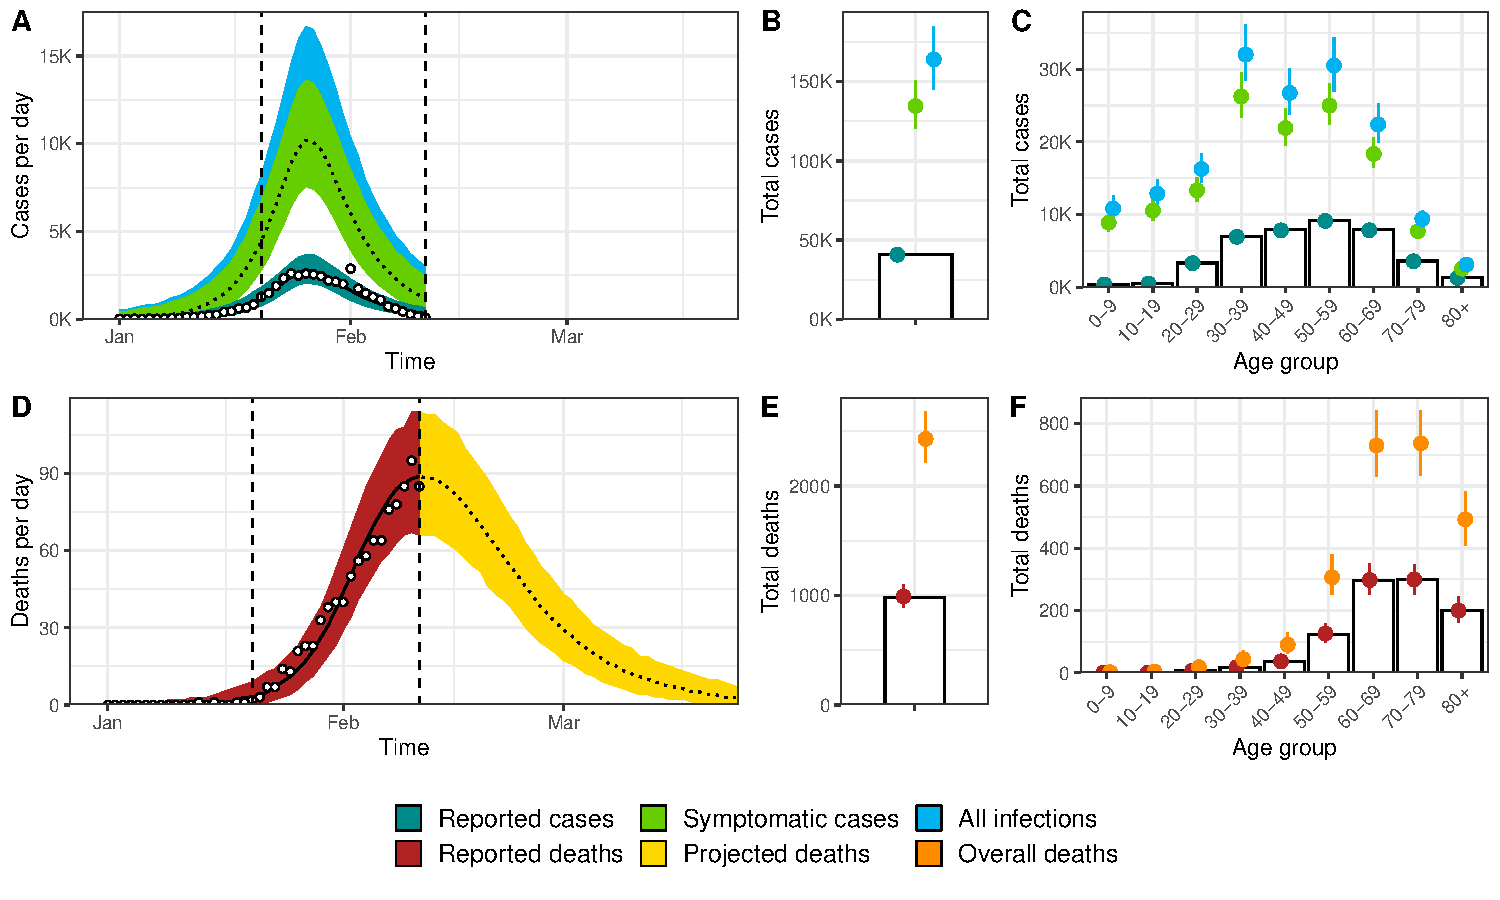
\includegraphics[width=\linewidth]{../format_output/figures/modelfit_china_rho50.pdf}
		\caption{Model fit for Hubei, China \textbf{with a fixed ascertainment proportion of older symptomatic patients of 50\% instead of 100\%.} (A) Incident cases of SARS-CoV-2 infection by date of disease onset, (B) total cases, (C) age distribution of cases, (D) incidence of deaths, (E) total deaths and (F) age distribution of deaths. White circles and bars represent data. Lines and shaded areas or points and ranges show the posterior median and 95\% credible intervals for six types of model output: reported cases, symptomatic cases, overall cases (i.e. symptomatic and asymptomatic cases), reported deaths until 11 February 2020, projected deaths after 11 February 2020 and overall deaths.}
		\label{fig:fit_sst1}
	\end{figure}

\begin{figure}[H]
	\centering
	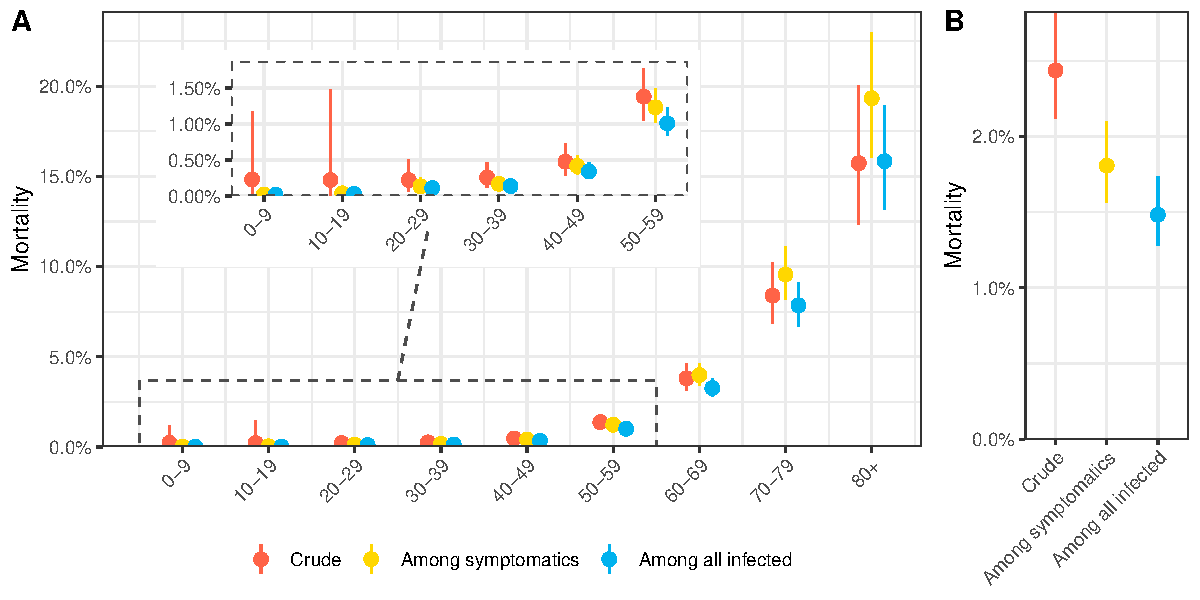
\includegraphics[width=.8\linewidth]{../format_output/figures/cfr_china_rho50.pdf}
	\caption{(A-B) Estimates of mortality during the first wave of the SARS-CoV-2 epidemic in Hubei, China by age group and overall \textbf{with a fixed ascertainment proportion of older symptomatic patients of 50\% instead of 100\%.} (C) Observed prevalence four comorbidities among deaths associated with SARS-CoV-2 infection in Hubei (purple) compared to the expected prevalence given the age distribution of deaths and the age-specific prevalence of each comorbidity in the Chinese population (white bar). Points and ranges show the posterior median and 95\% credible intervals.}
	\label{fig:mortality_sst1}
\end{figure}

\clearpage
\subsection{Reduced time between disease onset and death}

In the main analysis, the delay between disease onset and death was implemented using a log-normal distribution with mean 20.2 days and standard deviation 11.6. In this sensitivity analysis, we ran the analysis in Hubei using instead a log-normal distribution with mean 15 days and standard deviation 10. This resulted in a worse fit to data and less convincing external validation (Figure \ref{fig:fit_sst2}D).

\begin{figure}[H]
	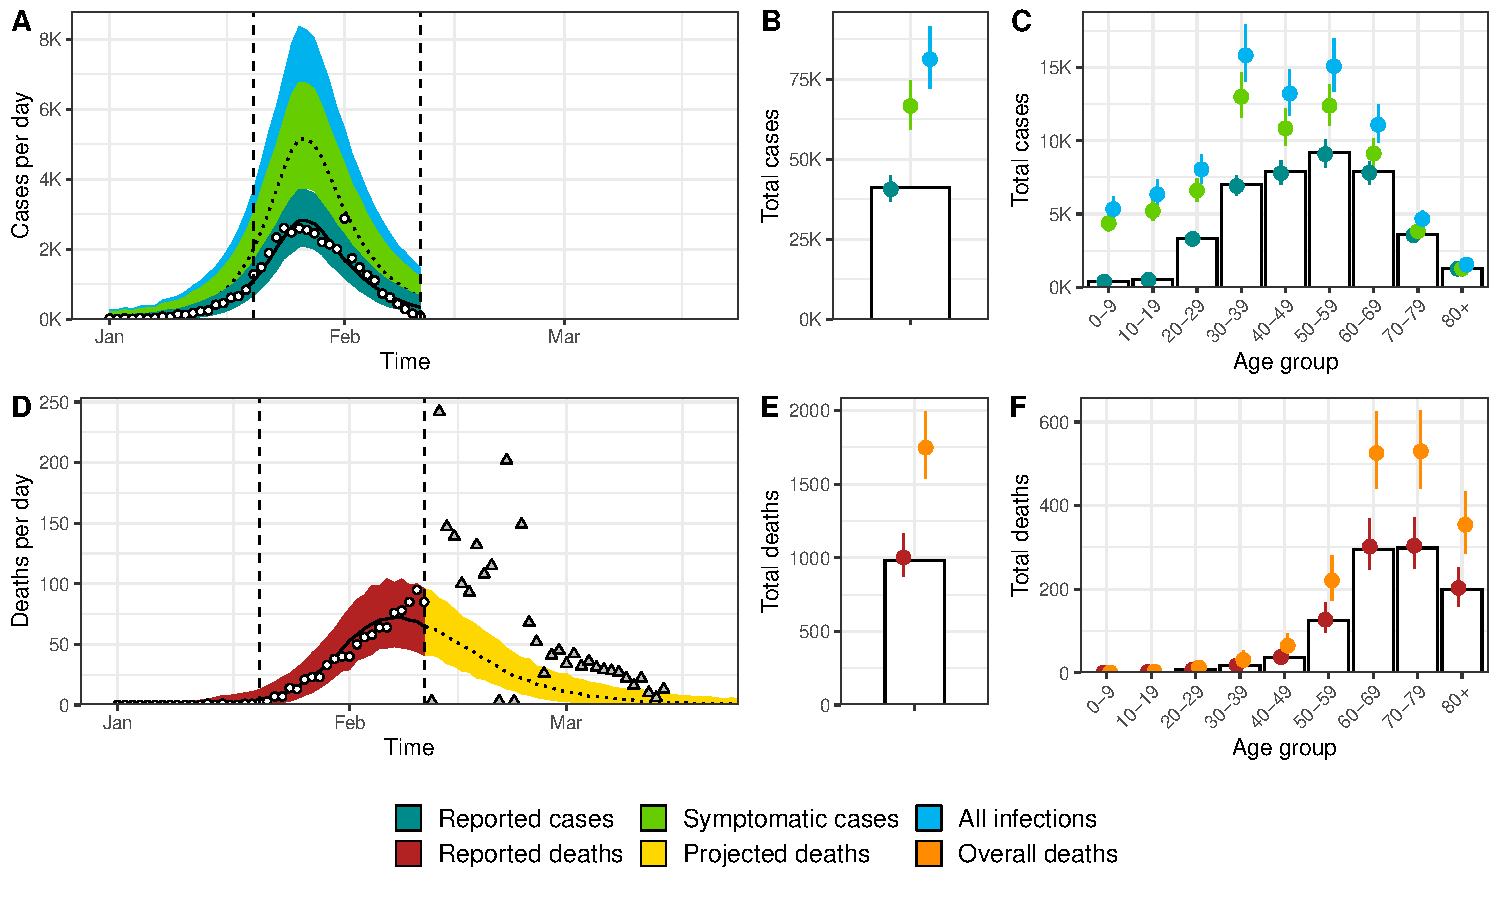
\includegraphics[width=\linewidth]{../format_output/figures/modelfit_china_gamma15.pdf}
	\caption{Model fit for Hubei, China \textbf{with a time between disease onset and death of 15 days on average instead of 20.2 days.} (A) Incident cases of SARS-CoV-2 infection by date of disease onset, (B) total cases, (C) age distribution of cases, (D) incidence of deaths, (E) total deaths and (F) age distribution of deaths. White circles and bars represent data. Lines and shaded areas or points and ranges show the posterior median and 95\% credible intervals for six types of model output: reported cases, symptomatic cases, overall cases (i.e. symptomatic and asymptomatic cases), reported deaths until 11 February 2020, projected deaths after 11 February 2020 and overall deaths.}
	\label{fig:fit_sst2}
\end{figure}


\clearpage
\section{Stan code}
\label{code}

Also available as \texttt{model13.stan} on \underline{\smash{\url{https://github.com/jriou/covid_adjusted_cfr/}}}.

\begin{verbatim}
functions {
real switch_eta(real t, real t1, real eta, real nu, real xi) {
return(eta+(1-eta)/(1+exp(xi*(t-t1-nu))));
}
real[] SEIR(real t,
real[] y,
real[] theta,
real[] x_r,
int[] x_i
) {
int K = x_i[1];

real tswitch = x_r[1];
real dydt[(4*K)]; //SEIAR, then C and D
real nI; // total infectious
real ntot;

real beta; // transmission rate
real eta; // reduction in transmission rate after quarantine
real xi; // slope of quarantine implementation
real nu; // shift of quarantine implementation
real tau; // incubation period
real mu; // infectious period
real psi; // probability of symptoms
real p_tswitch;
real contact[K*K];//contact matrix
real n_by_age[K];
real f_inf[K];

real init[K*4];
real age_dist[K];
real pi; // number of cases at t0

// estimated parameters
beta = theta[1];
eta = theta[2];
xi = theta[3];
nu = theta[4];
pi = theta[5];
psi = theta[6];

// Initial conditions
for(k in 1:K){
age_dist[k] = x_r[3+K*K + k];
init[k] = age_dist[k] * (1-pi);
init[K+k] = age_dist[k] * pi;
init[2*K+k] = 0.0;
init[3*K+k] = 0.0;
}

// fixed parameters
tau = 1.0/x_r[2];
mu = 1.0/x_r[3];
contact = x_r[4:(3+K*K)];

//Total number of infectious people
p_tswitch = switch_eta(t,tswitch,eta,nu,xi);

//Force of infection by age classes: 
//beta * p_tswitch * sum((number of infected people by age) / (total number of people by age) * 
//(number of contact by age))
for(k in 1:K){
f_inf[k] = beta * p_tswitch * sum(to_vector(y[(2*K+1):(3*K)]) ./ to_vector(age_dist) .* 
to_vector(contact[(K*(k-1)+1):(k*K)])); //
}
//print("Force of infection",f_inf);

for (k in 1:K) {
// S
dydt[k] = - f_inf[k] * (y[k]+init[k]); 
// E
dydt[K+k] = f_inf[k] * (y[k]+init[k])- tau * (y[K+k]+init[K+k]);
// I
dydt[2*K+k] = psi * tau * (y[K+k]+init[K+k]) - mu * (y[2*K+k]+init[2*K+k]);
// C
dydt[3*K+k] = psi * tau * (y[K+k]+init[K+k]);
}
return(dydt);
}
}

data {
int K; //number of age classes
vector[K] age_dist;
int pop_t; //total population
real tswitch;

//Data to fit
int D; //number of days with reported incidence
int incidence_cases[D]; //overal incidence for W weeks
int incidence_deaths[D]; //overal incidence for W weeks
int agedistr_cases[K]; //number of cases at tmax for the K age classes
int agedistr_deaths[K]; //mortality at tmax for the K age classes
//Parameters in priors
real p_beta;
real p_eta[2];
real p_pi[2];
real p_epsilon[2];
real p_rho[2];
real p_phi;
real p_xi;
real p_nu;
real p_psi[2];
// fixed parameters
real p_incubation;
real p_infectious;
int G;
real p_gamma[G];
//Simulation
real t0; //starting time
int t_data; //time of first data
int S;
real ts[S]; // time bins
real contact[K*K];

int inference;
int doprint;
}

transformed data {
real x_r[3+K*K+K]; //4 parameters + K*K contact matrix parameters + K age_dist parameters
int x_i[1] = {K};
real init[K*4] = rep_array(0.0, K * 4); // initial values
x_r[1] = tswitch;
x_r[2] = p_incubation;
x_r[3] = p_infectious;
x_r[4:(3+K*K)] = contact;
for(k in 1:K) {
x_r[3 + K*K + k] = age_dist[k];
}
}

parameters{
real<lower=0,upper=1> beta; // base transmission rate
real<lower=0,upper=1> eta; // reduction in transmission rate after quarantine measures
vector<lower=0,upper=1> [K] epsilon; // age-dependent mortality probability
vector<lower=0,upper=1> [K-1] raw_rho; // age-dependent reporting probability
real<lower=0, upper=1> pi; // number of cases at t0
real<lower=0> phi[2]; // variance parameters
real<lower=0,upper=1> xi_raw; // slope of quarantine implementation
real<lower=0> nu; // shift of quarantine implementation
real<lower=0,upper=1> psi; // proportion of symptomatics
}
transformed parameters {
// transformed parameters
vector[K] rho;
real xi = xi_raw+0.5;
// change of format for integrate_ode_rk45
real theta[6]; // vector of parameters
real y[S,K*4]; // raw ODE output
vector[K] comp_S[S];
vector[K] comp_E[S];
vector[K] comp_I[S];
vector[K] comp_D[S];
vector[K] comp_diffD[S];
vector[K] comp_C[S+G];
vector[K] comp_diffC[S+G];
vector[K] comp_diffM[S+G];
vector[K] comp_M[S+G];
// outcomes
vector[D] output_incidence_cases; // overall case incidence by day
vector[D] output_incidence_deaths; // overal mortality incidence by day 
simplex[K] output_agedistr_cases; // final age distribution of cases
simplex[K] output_agedistr_deaths; // final age distribution of deaths

// transformed paremeters
for(i in 1:(K-1)){
rho[i]=raw_rho[i];
}
rho[K] = 1.0;
// change of format for integrate_ode_rk45
theta[1:6] = {beta,eta,xi,nu,pi,psi};
// run ODE solver
y = integrate_ode_bdf(
SEIR, // ODE function
init, // initial states
t0, // t0
ts, // evaluation dates (ts)
theta, // parameters
x_r, // real data
x_i, // integer data
1.0E-10, 1.0E-10, 1.0E3); // tolerances and maximum steps
// extract and format ODE results (1.0E-9 correction to avoid negative values due to unprecise estimates
// of zeros as tolerance is 1.0E-10)
for(i in 1:S) {
comp_S[i] = (to_vector(y[i,1:K]) + to_vector(age_dist) * (1-pi) + 1.0E-9) * pop_t;
comp_E[i] = (to_vector(y[i,(K+1):(2*K)]) + to_vector(age_dist) * pi + 1.0E-9) * pop_t;
comp_I[i] = (to_vector(y[i,(2*K+1):(3*K)]) + 1.0E-9) * pop_t;

comp_C[i] = (to_vector(y[i,(3*K+1):(4*K)]) + 1.0E-9) * pop_t;
// lagged difference of cumulative incidence of symptomatics
comp_diffC[i] = i==1 ? comp_C[i,] : 1.0E-9*pop_t + comp_C[i,] - comp_C[i-1,]; 
}
//Incidence and cumulative incidence after S
for(g in 1:G){
comp_C[S+g] = comp_C[S];
comp_diffC[S+g] = rep_vector(1.0E-9,K);
}
//Mortality
//set diffM and M to 0
for(i in 1:(G+S)){
comp_diffM[i] = rep_vector(1.0E-9,K);
}
//compute mortality
for(i in 1:S) {
for(g in 1:G) {
comp_diffM[i+g] += comp_diffC[i] .* epsilon * p_gamma[g] ;
}
}
// cumulative sum
for(i in 1:(S+G)) {
for(k in 1:K) {
comp_M[i,k] = sum(comp_diffM[1:i,k]);
}
}
//compute D and diffD
for(i in 1:S){
comp_D[i] = (1.0-psi)/psi * comp_C[i];
comp_diffD[i] = (1.0-psi)/psi * comp_diffC[i];
}
// compute outcomes (again, 1.0E-9 correction to avoid negative values in the lagged differences)
for(i in t_data:S){
output_incidence_cases[i-t_data+1] = sum(comp_diffC[i].*rho);
output_incidence_deaths[i-t_data+1] = sum(comp_diffM[i]);
}
output_agedistr_cases = (comp_C[S,].*rho) ./ sum(comp_C[S,].*rho);
output_agedistr_deaths = (comp_M[S,]) ./ sum(comp_M[S,]);
}
model {
// priors
beta ~ beta(p_beta,p_beta);
eta ~ beta(p_eta[1],p_eta[2]);
for(k in 1:K) epsilon[k] ~ beta(p_epsilon[1],p_epsilon[2]);
for(k in 1:(K-1)) raw_rho[k] ~ beta(p_rho[1],p_rho[2]);
pi ~ beta(p_pi[1],p_pi[2]);
phi ~ exponential(p_phi);
xi_raw ~ beta(p_xi,p_xi); 
nu ~ exponential(p_nu);
psi ~ beta(p_psi[1],p_psi[2]);
// debug
if(doprint==1) {
print("beta: ",beta);
print("eta: ",beta);
print("epsilon: ",epsilon);
print("rho: ",rho);
print("pi: ",pi);
print("y[5,]: ",y[5,]);
print("comp_C[5,]: ",comp_C[5,]);
print("comp_diffC[5,]: ",comp_diffC[5,]);
print("comp_M[5,]: ",comp_M[5,]);
print("comp_diffM[5,]: ",comp_diffM[5,]);
}
// likelihood
if (inference==1) {
for(i in 1:D) {
target += neg_binomial_2_lpmf( incidence_cases[i] | output_incidence_cases[i], 
	output_incidence_cases[i]/phi[1]);
target += neg_binomial_2_lpmf( incidence_deaths[i] | output_incidence_deaths[i],
	output_incidence_deaths[i]/phi[2]);
}
target += multinomial_lpmf(agedistr_cases | output_agedistr_cases);
target += multinomial_lpmf(agedistr_deaths | output_agedistr_deaths);
}
}
\end{verbatim}

\bibliography{sup_bib}
	
\end{document}